




\subsection{Accuracy}
\label{eval-accu}



% ------- for next section
\def \fff        {$f$}
\def \flaps      {\textit{\#flaps}\xspace}
\def \gosLast    {$T_{lastGossip}$\xspace}
\def \gosAvg     {$T_{avgGossip}$\xspace}
\def \gosProc    {$T_{gossipExec}$\xspace}
\def \supProc    {$T_{stateUpdate}$\xspace}
\def \hops       {\textit{\#hops}\xspace}

\def \ringTable  {$Size_{ringTable}$\xspace}
\def \newStates  {$Size_{newStates}$\xspace}
\def \cpuSpeed   {$CPU$\xspace}




% d) $T_{avghbperiod}$ = h(all previous $T_{hbsilence}$) \\



\def \fgap {~~~~~~~~~~}
\def \fgap {~~~~}


\begin{figure}

\small
\centering


\begin{spacing}{1.5}
\begin{tabular}{|p{3.2in}|}
\hline

a) \flaps = \fff $($ \phi $>$ $8$ $)$ \\

b) \phi = \fff $($ \gosAvg, \gosLast $)$ \\
\fgap   \gosAvg = avg. of last 1000 \gosLast \\

c) \gosLast = \fff $($ \hops, \gosProc $)$ \\
\fgap \hops = $log(N)$ on average \\
\fgap \gosProc = \supProc (if new state changes) \\

d) \supProc = \fff $($ \ringTable, \newStates $)$ \\

\fgap   \ringTable $\leq$ $N$$\times$$P$ and \newStates $\leq$ $N$ \\



\hline
\end{tabular}
\end{spacing}

\vfive % orphan : we have extra space on page 10

\mycaption{fig-form}{Cassandra internal metrics (\sec\ref{eval-accu})}{Above
are the metrics we measured within the Cassandra bootstrap protocol
for measuring \sck accuracy (Figure \ref{fig-accu}). 
``f'' represents ``a function of'' (\ie, an arbitrary function).}


\end{figure}









Next, we provide a detailed accuracy evaluation of \sck.  Due to space
constraints, this section only focuses on one bug (Cassandra \caone
\cite{CA-One}, as described earlier in Figure \sec\ref{fig-mot}).  The
next section (\sec\ref{eval-bugs}) will summarize the other bugs we reproduced.


% metrics
Figure \ref{fig-form}a-d presents the  internal metrics within
Cassandra failure detection protocol that we measured for {\em every pair}
of nodes.  That is, the algorithm runs on every node A for every peer B.
%
Figures \ref{fig-accu}a-d compare in detail the accuracy of \stest without
PIL (``\ts{SCk}'') and \stestp with PIL (``\ts{SCk+PIL}'') compared to
the real deployments (``\ts{Real}'').
%
For example, $x$$=$512 implies the comparison of 512-node colocation in
\sck versus a real deployment of 512 nodes.



% ------------------------ a
Figure \ref{fig-accu}a shows the total number of flaps (alive-to-dead
transitions) observed in the whole cluster during bootstrapping.  
As described in the introduction of \sec\ref{sc-pil}, 
\stest by itself will not be accurate if all nodes are CPU intensive. 
%
However, with PIL, \sck closely mimics real deployment scenarios.  Most
importantly here, a significant \flaps does not appear until 256-node
deployment, hence techniques such as small/medium-scale testing or
mini-cluster extrapolation are not sufficient (\sec\ref{sec-rel}).
%
Next, Figure \ref{fig-form}a defines that \flaps depends on \phi
\cite{Hayashibara+04-PhiFailureDetector}.  Every node A maintains a \phi
value for a peer node B (a total of $N$$\times$$(N$$-$$1)$ variables to
monitor).  If \phi$>$8 for B, A will declare B dead (a flap).




% ------------------------ b
Figure \ref{fig-accu}b shows the maximum \phi values observed for every
peer node; for graph clarity, from here on we only show with-PIL results.
%
For example, for the 512-node setup, the whisker plots show the
distribution of the maximum \phi values observed for each of the 512
nodes.  As shown, the larger the cluster, more \phi values exceeds the
threshold value of 8, hence the flapping.
%
Figure \ref{fig-form}b points that \phi depends on the average
inter-arrival time of when new gossips about B arrives at A (\gosAvg) and
the time since A heard the last gossip about B (\gosLast); the ``last
gossip'' is the last version number received (Figure \sec\ref{fig-mot}).
The point is that \gosLast should not be much higher than \gosAvg.






\def \fgw {2.7in}



\begin{figure}[t]

%\centerline{

%}



\centerline{
%\hmina
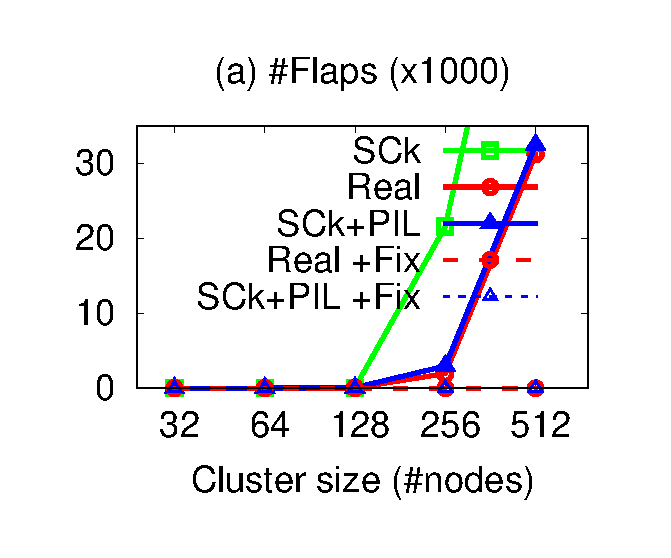
\includegraphics[width=\fgw]{F/accu/eps/flap}
%\hminb
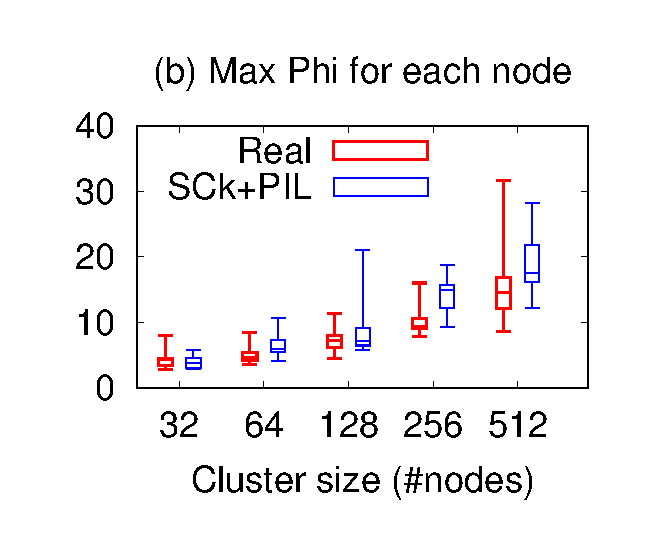
\includegraphics[width=\fgw]{F/accu/eps/phi}
%\hmina
%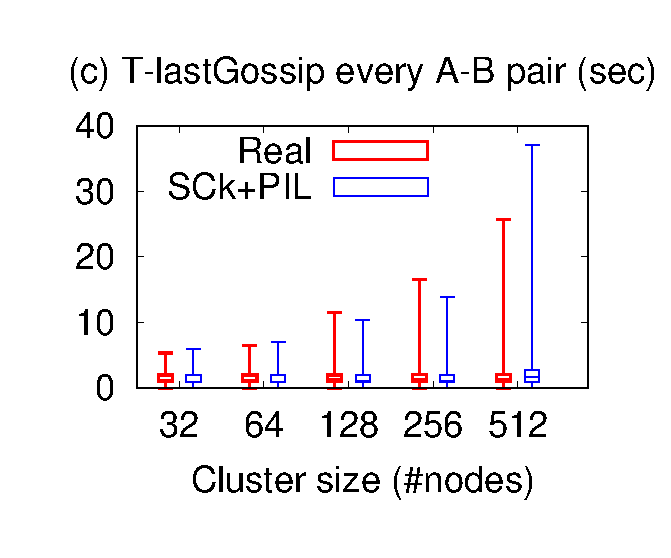
\includegraphics[width=\fgw]{F/accu/eps/hb}
%\hminb
%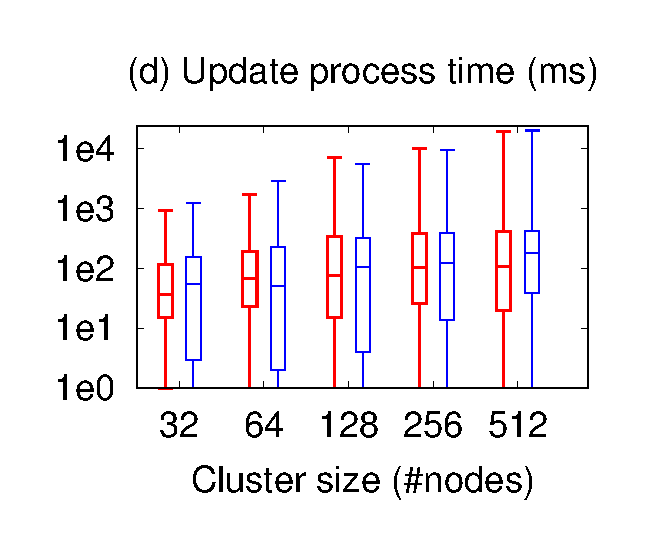
\includegraphics[width=\fgw]{F/accu/eps/proc-log}
}

%\vfive % orphan : we have extra space on page 10

\centerline{
%\hmina
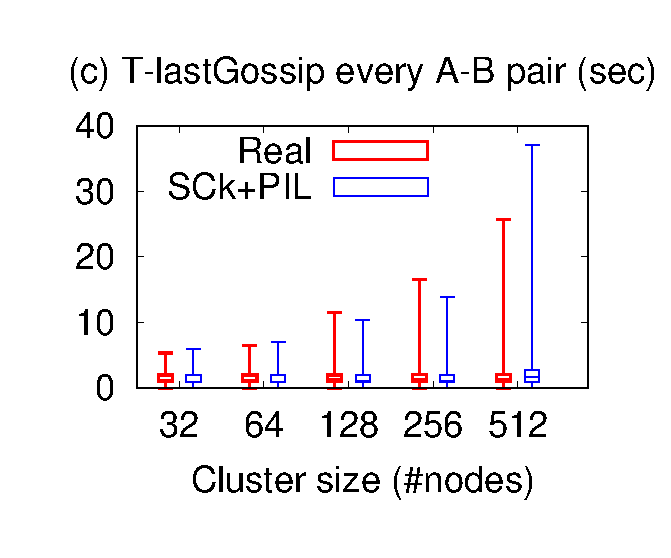
\includegraphics[width=\fgw]{F/accu/eps/hb}
%\hminb
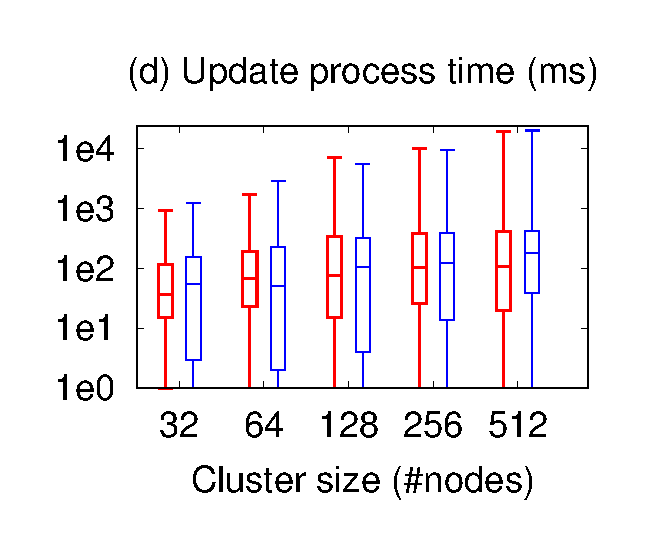
\includegraphics[width=\fgw]{F/accu/eps/proc-log}
}

%\centerline{
%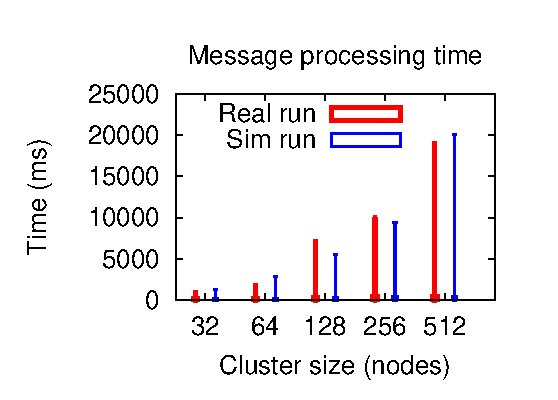
\includegraphics[width=\fgw]{F/accu/eps/proc}
%\includegraphics[width=\fgw]{F/accu/eps/hop}
%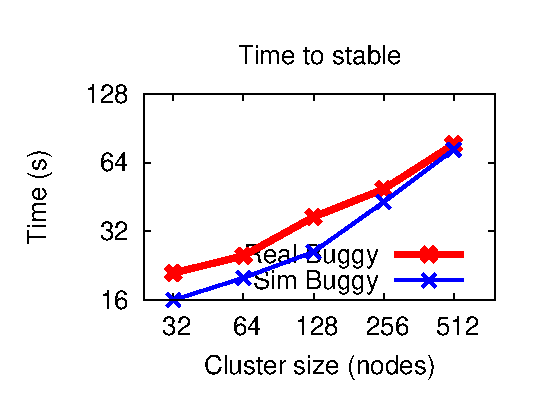
\includegraphics[width=\fgw]{F/accu/eps/stable}
%}

\vminten
\mycaption{fig-accu}{Accuracy in reproducing \caone (\sec\ref{eval-accu})}{The 
figures represent the metrics presented in Figure \ref{fig-form},
measured in real deployment (``Real'') and \sck with
different cluster sizes (32, 64, 128, 256, and 512).
Figure title represents the y-axis.}
\vminfive
\end{figure}




\if 0

\hsg{ b - 512
 c - 41295431
 d - 24335
recap, exampe, how many data points.
}

% \includegraphics[width=\fgw]{F/graphs/ca-6127/tsilent_99}
% \includegraphics[width=\fgw]{F/graphs/ca-6127/avgtsilent_99}
\includegraphics[width=\fgw]{F/graphs/ca-6127/avgtsilent}
\includegraphics[width=\fgw]{F/graphs/ca-6127/hop}
\includegraphics[width=\fgw]{F/graphs/ca-6127/hop}
\includegraphics[width=\fgw]{F/graphs/ca-6127/proctime}
\includegraphics[width=\fgw]{F/graphs/ca-6127/proctime_99}
\includegraphics[width=\fgw]{F/graphs/ca-6127/commit}
\includegraphics[width=\fgw]{F/graphs/ca-6127/commit_99}
\includegraphics[width=\fgw]{F/graphs/ca-6127/profiling}
\includegraphics[width=\fgw]{F/graphs/ca-6127/table}
\includegraphics[width=\fgw]{F/graphs/ca-6127/table_med}
\fi



% ------------------------ c
Figure \ref{fig-accu}c shows the whisker plots of gossip inter-arrival
times (\gosLast) that we collected for every A-B pair.  For example, for
the 512-node setup, the whisker plots represent the distribution of around
41 million gossip inter-arrival times; this large number is because a
message contains gossips of many peer nodes.  The figure shows that in
larger clusters, new gossips do not arrive as fast as in smaller clusters,
especially at high percentiles.
%
Figure \ref{fig-form}c shows that \gosLast depends on how far B's new
gossips propagate through other nodes to A (\hops) and the gossip
processing time in each hop (\gosProc).  The \hops is stable
at $log(N)$ on average in \sck and real deployment (not shown).  The
latter (\gosProc) is essentially state-update processing time (\supProc)
whenever there are state changes, which is the culprit.

% ------------------------ d
Figure \ref{fig-accu}d ({\em in log scale}) shows the whisker plots of
state-update processing time (\supProc); in the 512-node setup, we
measured around 25,000 state-update invocations.  The figure shows that at
high percentiles, \supProc is scale-dependent.  As shown in Figure
\ref{fig-form}d, \supProc complicatedly
depends on a scale-dependent 2-dimensional input (\ringTable and
\newStates); a node's \ringTable depends on how many nodes it knows,
including the partition arrangement ($\leq$$N$$\times$$P$) and \newStates
($\leq$$N$), which increases as cluster size increases.
%
%The bug was not expected because the median of \supProc is not
%scale-dependent.
%





We conclude that PIL-infused \sck mimics similar behaviors as in real
deployments and is accurate for reproducing scalability bugs.
%
As an additional note, we have applied the fix patch in both \sck (without
redoing memoization) and real deployment modes; Figure \ref{fig-accu}a
shows \flaps is always zero in both modes (``\ts{+Fix}'' lines).



